\chapter{Análisis de Desempeño y Benchmarking}

Para evaluar de forma rigurosa el rendimiento de las cuatro implementaciones desarrolladas, se diseñó un benchmarking script que somete a cada versión del programa a seis configuraciones distintas de trabajo computacional, combinando tres resoluciones de imagen ($800 \times 800$, $2000 \times 2000$ y $5000 \times 5000$~píxeles) con dos perfiles de filtrado: un \textit{perfil liviano} (filtro de $3 \times 3$ con 3~niveles de posterizado) y un \textit{perfil pesado} (filtro de $5 \times 5$ con 9~niveles de posterizado). Cada configuración se ejecutó durante 10~iteraciones consecutivas para obtener muestras estadísticamente representativas. Las pruebas se realizaron sobre un clúster donde OpenMP utilizó 32~núcleos dentro de un único nodo, mientras que MPI y la versión Híbrida emplearon 128~núcleos distribuidos en 4~nodos ($4\ \mathit{nodos} \times 32\ \mathit{cores}$).

A continuación se presenta el análisis detallado de cada escenario, seguido de una comparación general, las curvas de \textit{Speedup} y \textit{Eficiencia}, y un estudio de escalabilidad en función de la cantidad de hilos.


%--------------------------------------------------------------------
\section{Imagen de \texorpdfstring{$800 \times 800$}{800x800} píxeles}

\subsection{Configuración: filtro \texorpdfstring{$3 \times 3$}{3x3}, 3 niveles}

\begin{figure}[H]
    \centering
    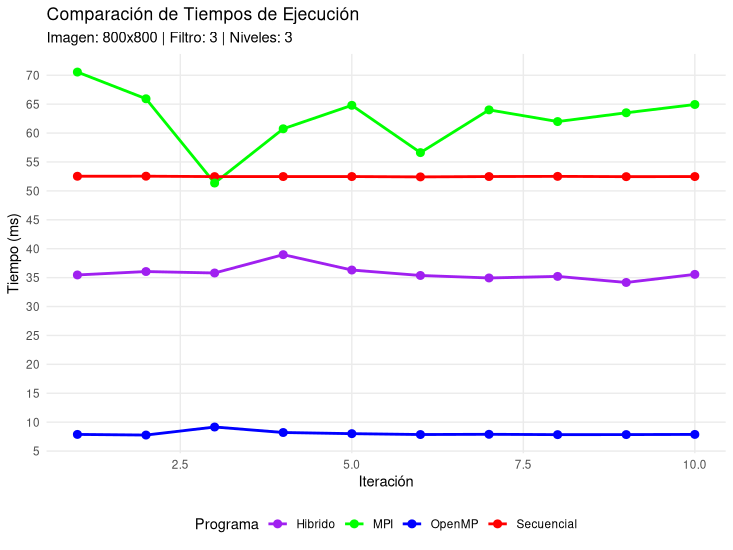
\includegraphics[width=0.85\textwidth]{../resources/800_3_3.png}
    \caption{Comparación de tiempos de ejecución --- Imagen $800 \times 800$, filtro $3 \times 3$, 3~niveles de posterizado.}
    \label{fig:800_3_3}
\end{figure}

En la configuración más liviana del benchmark, la carga computacional resulta extremadamente reducida: la versión secuencial completa el pipeline en aproximadamente 52~ms de forma estable a lo largo de las 10~iteraciones. OpenMP demuestra una aceleración notable, reduciendo los tiempos a cerca de 8~ms con una variabilidad mínima entre iteraciones. Sin embargo, la versión MPI exhibe el comportamiento más desfavorable de los cuatro modelos, con tiempos que oscilan entre 51~ms y 71~ms, superando incluso a la versión secuencial en la mayoría de las iteraciones. Este resultado evidencia que, para un volumen de datos reducido ($800 \times 800 = 640{.}000$~píxeles), el \textit{overhead} inherente a la comunicación por red (distribución mediante \texttt{MPI\_Scatterv}, intercambio de halos y recolección con \texttt{MPI\_Gatherv}) supera al beneficio obtenido por la paralelización del cómputo entre los 128~núcleos. La versión Híbrida se posiciona en un punto intermedio, con tiempos alrededor de 35~ms: si bien logra reducir el tiempo respecto de la versión secuencial gracias al cómputo paralelo interno con OpenMP, aún arrastra la penalización de la coordinación entre los 4~nodos MPI.


\subsection{Configuración: filtro \texorpdfstring{$5 \times 5$}{5x5}, 9 niveles}

\begin{figure}[H]
    \centering
    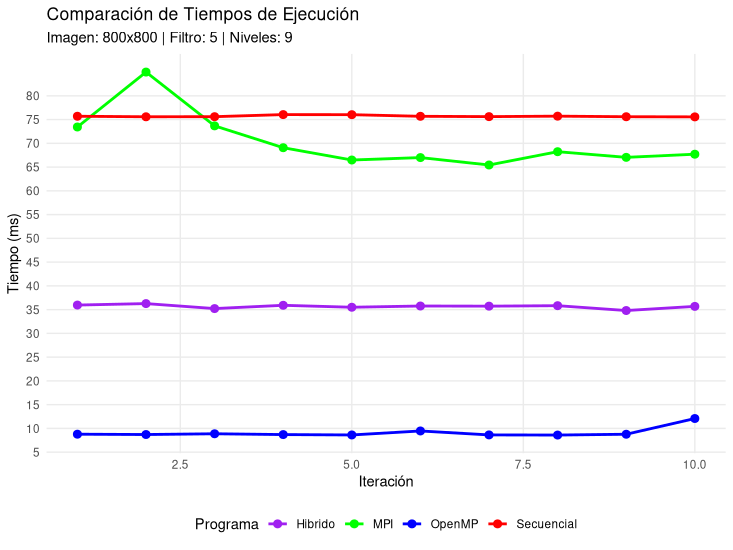
\includegraphics[width=0.85\textwidth]{../resources/800_5_9.png}
    \caption{Comparación de tiempos de ejecución --- Imagen $800 \times 800$, filtro $5 \times 5$, 9~niveles de posterizado.}
    \label{fig:800_5_9}
\end{figure}

Al incrementar la complejidad del filtrado (kernel de $5 \times 5$, que implica 25~operaciones por píxel en lugar de 9, y 9~niveles de posterizado), los tiempos secuenciales ascienden a aproximadamente 76~ms. OpenMP continúa liderando con tiempos cercanos a 9~ms, prácticamente sin degradación respecto de la configuración anterior. La versión MPI se mantiene cercana a los tiempos del modelo secuencial, oscilando entre 65~ms y 85~ms, pero por debajo respecto de la línea base secuencial en la mayoría de iteraciones, logrando una aceleración positiva y justificando el costo de la comunicación entre los 128~procesos. La versión Híbrida mantiene su comportamiento estable alrededor de 36~ms, confirmando que el cuello de botella en esta resolución no es el cómputo sino la latencia de comunicación entre nodos.



%--------------------------------------------------------------------
\section{Imagen de \texorpdfstring{$2000 \times 2000$}{2000x2000} píxeles}

\subsection{Configuración: filtro \texorpdfstring{$3 \times 3$}{3x3}, 3 niveles}

\begin{figure}[H]
    \centering
    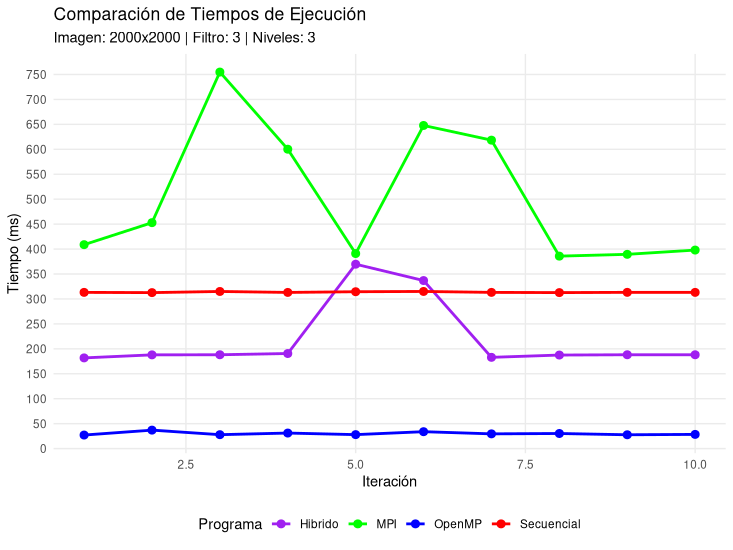
\includegraphics[width=0.85\textwidth]{../resources/2000_3_3.png}
    \caption{Comparación de tiempos de ejecución --- Imagen $2000 \times 2000$, filtro $3 \times 3$, 3~niveles de posterizado.}
    \label{fig:2000_3_3}
\end{figure}

Con una imagen de resolución intermedia ($2000 \times 2000 = 4{.}000{.}000$~píxeles), las diferencias entre los paradigmas comienzan a acentuarse. La versión secuencial se mantiene estable aproximadamente en torno a 315~ms. OpenMP reduce drásticamente este tiempo a un rango de 25--40~ms, demostrando una escalabilidad sólida al aumentar el tamaño del problema. La versión MPI, en cambio, tiene una alta inestabilidadm, con tiempos que fluctúan entre 385~ms y 755~ms, y con picos que casi duplican el tiempo secuencial; esta variabilidad se le puede atribuir a la congestión de red. La versión Híbrida presenta un comportamiento interesante: en la mayoría de las iteraciones se mantiene alrededor de 188~ms y por debajo de la línea base secuencial, pero en las iteraciones 5 y 6 se observan picos de hasta 370~ms, posiblemente causados por interferencia puntual en la red del clúster.


\subsection{Configuración: filtro \texorpdfstring{$5 \times 5$}{5x5}, 9 niveles}

\begin{figure}[H]
    \centering
    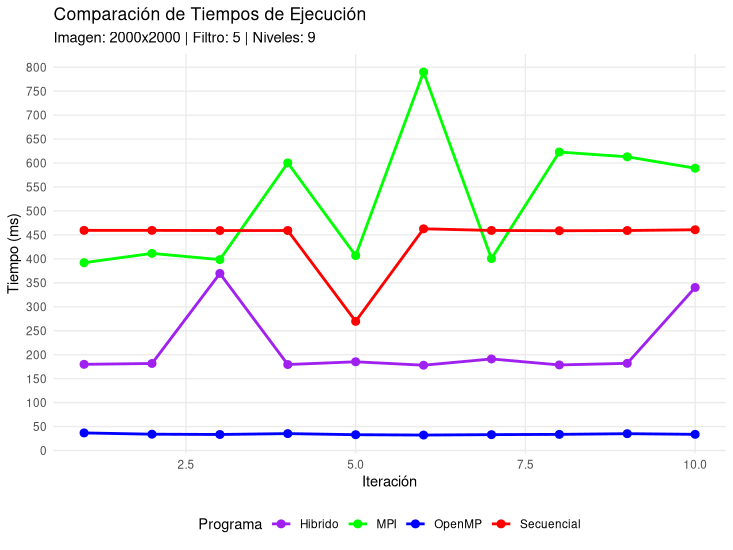
\includegraphics[width=0.85\textwidth]{../resources/2000_5_9.png}
    \caption{Comparación de tiempos de ejecución --- Imagen $2000 \times 2000$, filtro $5 \times 5$, 9~niveles de posterizado.}
    \label{fig:2000_5_9}
\end{figure}

El perfil pesado sobre la imagen de $2000 \times 2000$ eleva el tiempo secuencial a aproximadamente 460~ms, con un valor anómalo en la iteración~5 de 270~ms, probablemente causado por un efecto de caché favorable en esa ejecución particular. OpenMP mantiene tiempos consistentemente bajos entre 35~ms y 40~ms, demostrando que la mayor carga aritmética del kernel de $5 \times 5$ se paraleliza sin degradación apreciable. MPI presenta su peor comportamiento en esta configuración, con picos que alcanzan los 790~ms, practicamente duplicando el tiempo secuencial, y una dispersión considerable entre iteraciones (rango de 390~ms a 790~ms). La versión Híbrida se mantiene generalmente estable cerca de 180~ms, aunque nuevamente se observan picos esporádicos (iteraciones 3 y 10 por encima de 340~ms), coherentes con el patrón de interferencia de red observado.


%--------------------------------------------------------------------
\section{Imagen de \texorpdfstring{$5000 \times 5000$}{5000x5000} píxeles}

\subsection{Configuración: filtro \texorpdfstring{$3 \times 3$}{3x3}, 3 niveles}

\begin{figure}[H]
    \centering
    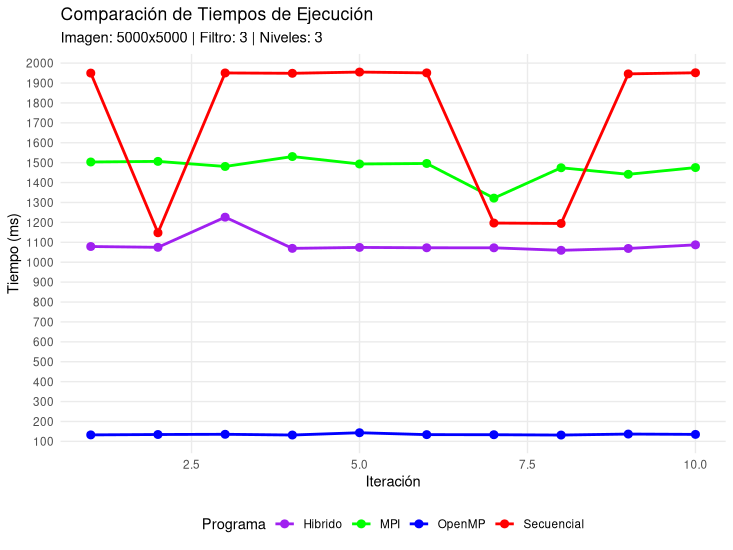
\includegraphics[width=0.85\textwidth]{../resources/5000_3_3.png}
    \caption{Comparación de tiempos de ejecución --- Imagen $5000 \times 5000$, filtro $3 \times 3$, 3~niveles de posterizado.}
    \label{fig:5000_3_3}
\end{figure}

Al alcanzar la resolución máxima del benchmark ($5000 \times 5000 = 25{.}000{.}000$~píxeles), el escenario cambia significativamente respecto de las resoluciones menores. La versión secuencial presenta tiempos alrededor de 1950~ms, con caídas a 1150--1200~ms en las iteraciones 2, 7 y 8 (atribuibles a efectos de caché). OpenMP continúa obteniendo los mejores tiempos, entre 130~ms y 140~ms. La observación más relevante en esta resolución es que MPI logra nuevamente superar a la versión secuencial con tiempos entre 1320~ms y 1530~ms, lo que indica que el volumen de cómputo de 25~millones de píxeles justifica el costo de la comunicación MPI. La versión Híbrida consolida su posición intermedia con tiempos alrededor de 1070~ms, superando tanto a la versión secuencial como a MPI, y confirmando que la reducción del tráfico de red (de 128 a solo 4~procesos MPI) combinada con el paralelismo local de OpenMP resulta una estrategia más eficiente que MPI puro.


\subsection{Configuración: filtro \texorpdfstring{$5 \times 5$}{5x5}, 9 niveles}

\begin{figure}[H]
    \centering
    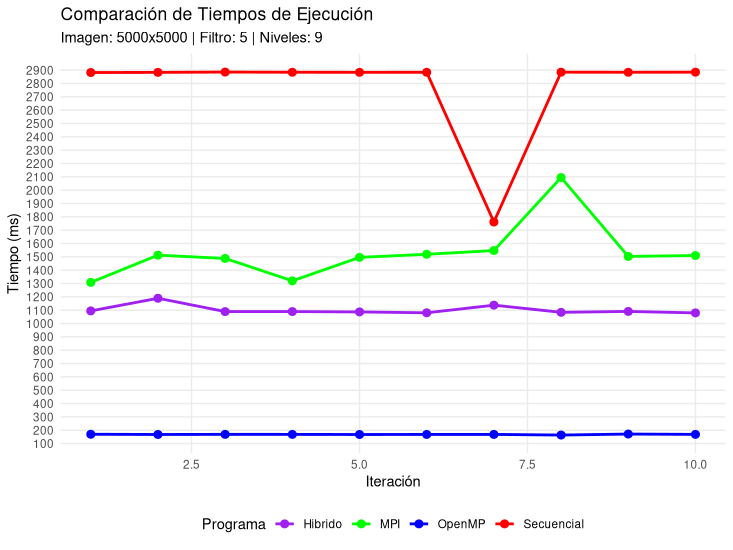
\includegraphics[width=0.85\textwidth]{../resources/5000_5_9.png}
    \caption{Comparación de tiempos de ejecución --- Imagen $5000 \times 5000$, filtro $5 \times 5$, 9~niveles de posterizado.}
    \label{fig:5000_5_9}
\end{figure}

La configuración más exigente del benchmark ($5000 \times 5000$ con kernel de $5 \times 5$ y 9~niveles) expone con máxima claridad la jerarquía de rendimiento entre las cuatro implementaciones. La versión secuencial alcanza los 2890~ms de forma estable, con una excepción en la iteración~7, que desciende a 1760~ms; nuevamente un caso atípico. OpenMP logra tiempos entre 160~ms y 170~ms; $10$ veces superior respecto del modelo secuencial. MPI mantiene tiempos entre 1310~ms y 1540~ms en la mayoría de las iteraciones, con un pico aislado de 2100~ms en la iteración~8, demostrando que, si bien la paralelización es efectiva a esta escala, la variabilidad introducida por la red sigue siendo un factor influyente. La versión Híbrida se estabiliza entre 1090~ms y 1190~ms, superando consistentemente tanto a la versión secuencial como a MPI puro, y posicionándose como la segunda opción más rápida después de OpenMP en un único nodo.


%--------------------------------------------------------------------
\section{Comparación General de Tiempos}

\begin{figure}[H]
    \centering
    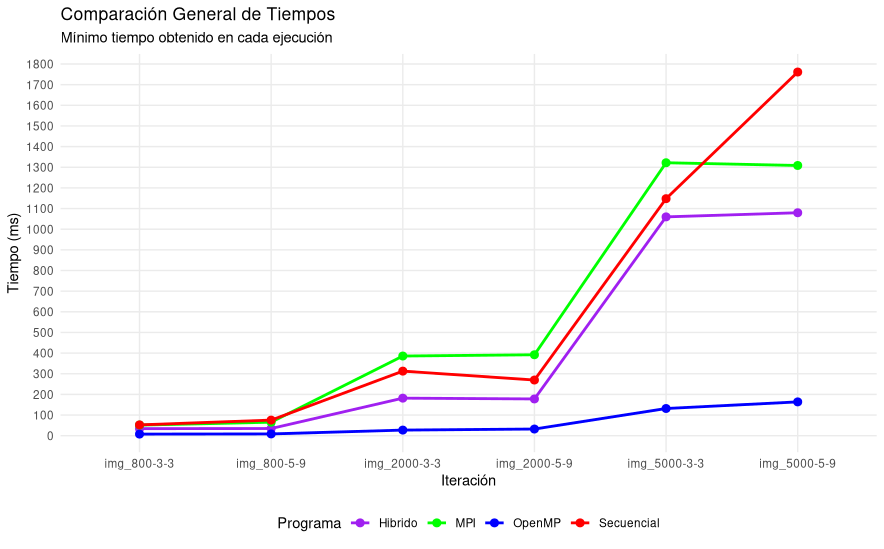
\includegraphics[width=0.9\textwidth]{../resources/Comp_General.png}
    \caption{Comparación general de tiempos --- Mínimo tiempo obtenido por cada implementación en las seis configuraciones de benchmark.}
    \label{fig:comp_general}
\end{figure}

La vista de los mejores tiempos obtenidos en cada configuración permite visualizar con claridad las tendencias de escalabilidad de cada paradigma. Para las resoluciones pequeñas ($800 \times 800$), los cuatro modelos operan en un rango temporal estrecho (entre 8~ms y 71~ms), donde la diferencia absoluta entre el mejor y el peor caso resulta poco significativa en términos prácticos. Sin embargo, a medida que la resolución crece, las curvas divergen drásticamente.

La versión Secuencial (línea roja) sirve como referencia superior, con un crecimiento lineal respecto del volumen de datos.

OpenMP (línea azul) se mantiene en la franja inferior del gráfico en todas las configuraciones, creciendo de forma suave y controlada: pasa de aproximadamente 8~ms en $800 \times 800$ a 160~ms en $5000 \times 5000$. Este crecimiento es proporcionalmente menor al aumento del volumen de datos, lo que demuestra una paralelización altamente eficiente dentro de un único nodo.

La versión Híbrida (línea morada) muestra un comportamiento intermedio consistente: su curva crece más lentamente que la de MPI, confirmando que reducir la cantidad de procesos MPI a solo 4 (uno por nodo) y delegar el paralelismo fino a OpenMP es una estrategia más escalable que utilizar MPI de forma exclusiva.

MPI (línea verde) exhibe la peor escalabilidad: si bien en algunas resoluciones sus tiempos superan a los de la versión secuencial, su curva crece de forma empinada y con alta variabilidad.


%--------------------------------------------------------------------
\section{Análisis de Speedup}

\begin{figure}[H]
    \centering
    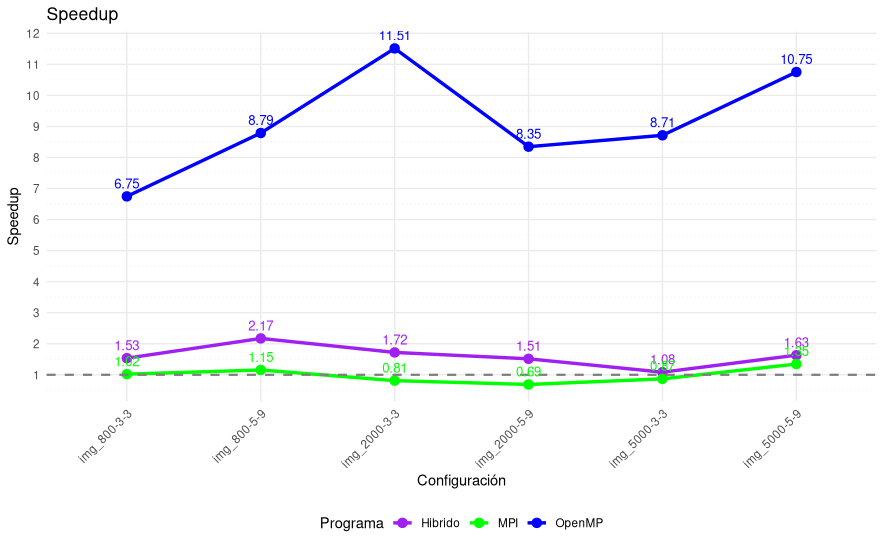
\includegraphics[width=0.9\textwidth]{../resources/Speedup.png}
    \caption{Speedup de las implementaciones paralelas respecto de la versión secuencial en las seis configuraciones de benchmark. La línea punteada indica $S = 1$ (sin aceleración).}
    \label{fig:speedup}
\end{figure}

Aquí podemos observar que OpenMP alcanza speedups considerablemente elevados durante todas las configuraciones, con un máximo de $11.51$ y un valor de $10.75$ en la configuración más exigente.

De MPI obtenemos el siguiente resultado: En tres configuraciónes obtiene ganancia (speedup mayor a 1), y en tres configuraciones no obtiene ganancia (speedup inferioir a 1), haciendo dificíl la elección de su implementación en un proyecto de esta escala.

La versión Híbrida logra speedups modestos comparados con OpenMP, pero superiores a MPI en todos los casos, oscilando entre $1.51$ y $2.17$. A pesar de ser resultados humildes, superan consistentemente la línea de $S = 1$, lo que demuestra que la combinación de ambos paradigmas resulta viable incluso cuando la escala del problema no favorece del todo a MPI puro.


%--------------------------------------------------------------------
\section{Análisis de Eficiencia}

\begin{figure}[H]
    \centering
    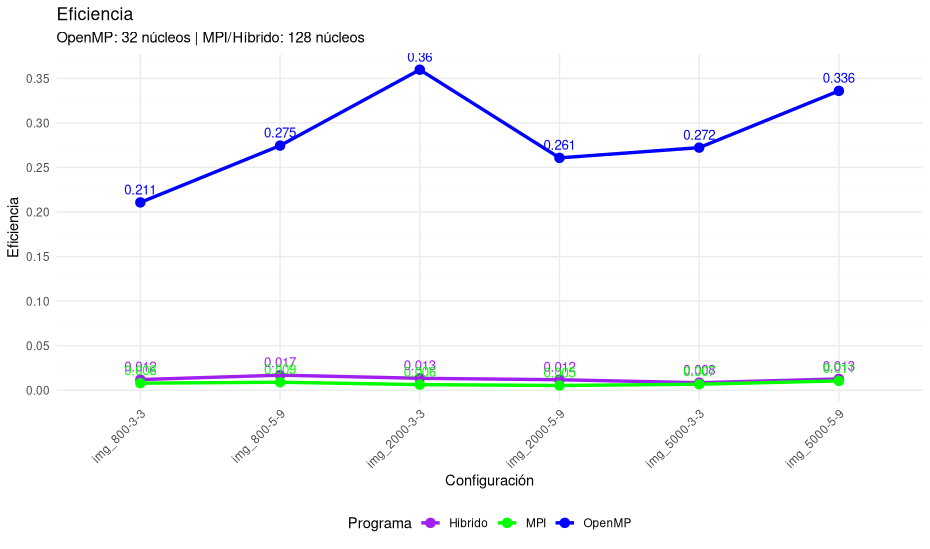
\includegraphics[width=0.9\textwidth]{../resources/Eficiencia.png}
    \caption{Eficiencia de las implementaciones paralelas. OpenMP utiliza 32~núcleos; MPI e Híbrido utilizan 128~núcleos.}
    \label{fig:eficiencia}
\end{figure}

Los resultados revelan una diferencia abismal en el aprovechamiento de los recursos. OpenMP, con 32~núcleos, alcanza eficiencias entre $0.211$ y $0.360$, lo que significa que entre el 21\% y el 36\% de la capacidad de cómputo se traduce en aceleración real.

En marcado contraste, MPI e Híbrido presentan eficiencias extremadamente bajas: entre $0{.}005$ y $0{.}017$ para MPI ($0{.}5\%$--$1{.}7\%$ de aprovechamiento) y entre $0{.}008$ y $0{.}017$ para Híbrido ($0{.}8\%$--$1{.}7\%$ de aprovechamiento). Estas cifras indican que la gran mayoría de los 128~núcleos asignados pasan una fracción dominante de su tiempo esperando comunicaciones de red, sincronizaciones de barrera o intercambios de halos, en lugar de realizar cómputo útil.

De este resultado podemos decir que: \textbf{Agregar más procesadores no siempre se traduce en mayor rendimiento} y, para este problema en particular, la configuración de 32~núcleos con memoria compartida (OpenMP) se posiciona como la opción más eficiente.


%--------------------------------------------------------------------
\section{Escalabilidad según Cantidad de Hilos}

Los análisis previos evaluaron el rendimiento de cada paradigma con una cantidad fija de unidades de procesamiento (32~hilos para OpenMP, 128~núcleos para MPI e Híbrido). Ahora nos toca observar cómo escala cada implementación al incrementar gradualmente los threads disponibles. Para ello, se diseñó un script el cuál varia la cantidad de hilos OpenMP utilizando la secuencia $\{1, 2, 4, 8, 16, 32\}$ (potencias de a dos), manteniendo fija la configuración computacionalmente más exigente del benchmark: imagen de $5000 \times 5000$~píxeles con filtro de $5 \times 5$ y 9~niveles de posterizado. ¿Por qué esta configuración? Maximizar el volumen de cómputo por píxel permite observar con mayor claridad la tendencia de escalabilidad.

Para la versión OpenMP, las 10~iteraciones de cada configuración se ejecutaron sobre un único nodo del clúster, variando exclusivamente el parámetro \texttt{-t} que controla la cantidad de threads. Para la versión Híbrida, se mantuvieron fijos los 4~procesos MPI (uno por nodo físico) y se varió la cantidad de hilos OpenMP internos de cada proceso. En ambos casos, el speedup se calculó de forma relativa a la ejecución con un único hilo del mismo programa ($S(p) = T(1) / T(p)$), lo que permite medir la ganancia neta atribuible exclusivamente al aumento de threads.


\subsection{Speedup según cantidad de hilos}

\begin{figure}[H]
    \centering
    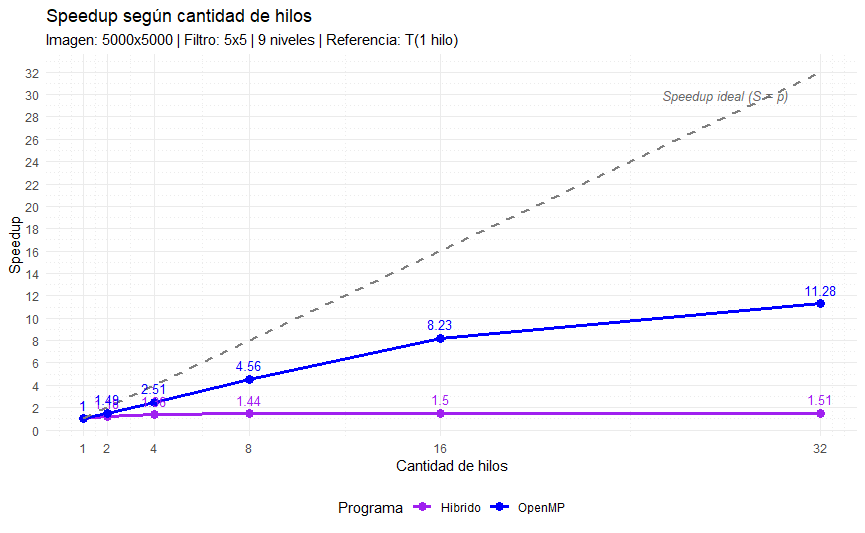
\includegraphics[width=0.9\textwidth]{../resources/Speedup_threads.png}
    \caption{Speedup en función de la cantidad de hilos para OpenMP e Híbrido. La línea punteada representa el speedup ideal ($S = p$). Configuración: imagen $5000 \times 5000$, filtro $5 \times 5$, 9~niveles.}
    \label{fig:speedup_threads}
\end{figure}

La curva de OpenMP (línea azul) exhibe un crecimiento sostenido y consistente a lo largo de todo el rango evaluado. Con 2~hilos se obtiene un speedup de $1{.}49$, lo que indica que prácticamente la totalidad del trabajo se distribuye efectivamente entre ambos hilos, con una pérdida mínima por overhead de creación del equipo de hilos. Al pasar a 4~hilos el speedup asciende a $2{.}51$, manteniendo una progresión cercana a la linealidad. El salto más significativo se produce al escalar a 8~hilos ($S = 4{.}56$), punto en el cual la curva comienza a separarse visiblemente de la línea de speedup ideal ($S = p$). La brecha entre la curva real y el speedup ideal demuestra el impacto de la fracción secuencial del algoritmo, acceso simultáneo a memoria, y el overhead propio de sincronización OpenMP.

La versión Híbrida (línea púrpura) presenta un comportamiento radicalmente distinto. Si bien con 2~hilos por nodo logra un speedup de $1{.}18$ respecto de su propia ejecución con 1~hilo, la curva se aplana casi por completo a partir de 4~hilos, estabilizándose en un rango estrecho entre $1{.}44$ y $1{.}51$ para todas las configuraciones de 4 a 32~hilos. Este estancamiento se explica por la latencia de la comunicación entre los 4~nodos MPI.


\subsection{Eficiencia según cantidad de hilos}

\begin{figure}[H]
    \centering
    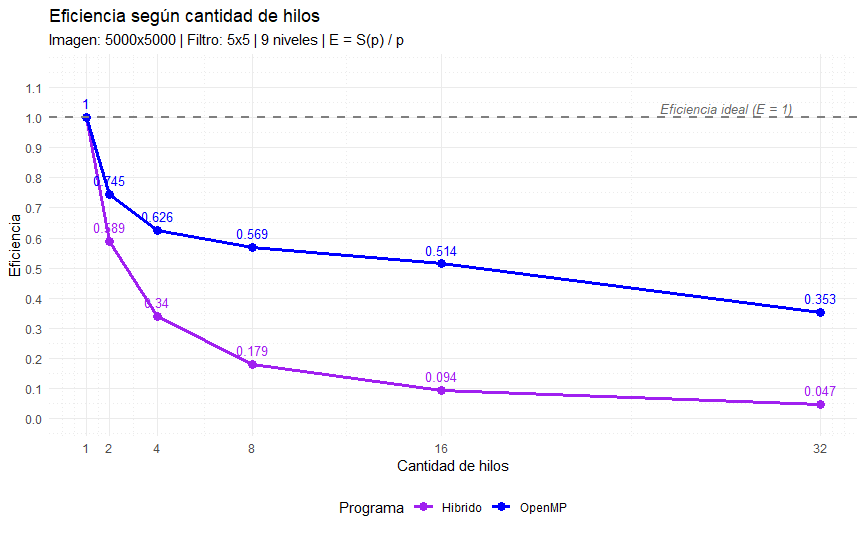
\includegraphics[width=0.9\textwidth]{../resources/Eficiencia_threads.png}
    \caption{Eficiencia en función de la cantidad de hilos para OpenMP e Híbrido. La línea punteada representa la eficiencia ideal ($E = 1$). Configuración: imagen $5000 \times 5000$, filtro $5 \times 5$, 9~niveles.}
    \label{fig:eficiencia_threads}
\end{figure}

OpenMP exhibe una degradación monótona pero controlada a medida que se incrementa la cantidad de hilos. Con 2~hilos la eficiencia se mantiene en $0{.}745$ (el $74{.}5\%$ del recurso agregado se aprovecha), desciende a $0{.}626$ con 4~hilos, y continúa cayendo de manera gradual hasta estabilizarse en $0{.}353$ con 32~hilos. El hecho de que con 32~hilos aún se conserve un $35{.}3\%$ de eficiencia confirma que el pipeline de procesamiento de imágenes posee una fracción paralela dominante, y que las decisiones de diseño adoptadas fueron efectivas.

En contraste, la versión Híbrida muestra una caída de eficiencia considerablemente más pronunciada. Desde un valor inicial de $0{.}589$ con 2~hilos, la eficiencia se desploma a $0{.}34$ con 4~hilos y continúa descendiendo hasta alcanzar apenas $0{.}047$ con 32~hilos por nodo (aprovechamiento del $4{.}7\%$). Esta degradación acelerada se explica por la asimetría inherente al modelo híbrido. A medida que el cómputo local se vuelve más rápido (aumento de hilos OpenMP), la fracción del tiempo total que se fue por la comunicación en red crece, haciendo que cada thread adicional aporte una mejora cada vez menor.